%%% Hlavní soubor. Zde se definují základní parametry a odkazuje se na ostatní části. %%%

%% Verze pro jednostranný tisk:
% Okraje: levý 40mm, pravý 25mm, horní a dolní 25mm
% (ale pozor, LaTeX si sám přidává 1in)
\documentclass[12pt,a4paper]{report}
\setlength\textwidth{145mm}
\setlength\textheight{247mm}
\setlength\oddsidemargin{15mm}
\setlength\evensidemargin{15mm}
\setlength\topmargin{0mm}
\setlength\headsep{0mm}
\setlength\headheight{0mm}
% \openright zařídí, aby následující text začínal na pravé straně knihy
\let\openright=\clearpage

%% Pokud tiskneme oboustranně:
% \documentclass[12pt,a4paper,twoside,openright]{report}
% \setlength\textwidth{145mm}
% \setlength\textheight{247mm}
% \setlength\oddsidemargin{15mm}
% \setlength\evensidemargin{0mm}
% \setlength\topmargin{0mm}
% \setlength\headsep{0mm}
% \setlength\headheight{0mm}
% \let\openright=\cleardoublepage

%% Pokud používáte csLaTeX (doporučeno):
%\usepackage{czech}
%% Pokud nikoliv:
\usepackage[slovak]{babel} % aby mi nepisalo Obrazek ;-)
%\usepackage[T1]{fontenc}

%% Použité kódování znaků: obvykle latin2, cp1250 nebo utf8:
\usepackage[utf8]{inputenc}

%% Ostatní balíčky
\usepackage{graphicx}
\usepackage{amsthm}
\usepackage{epstopdf}
\newtheorem{theorem}{Věta}
\newtheorem*{define}{Definice}	% Definice nečíslujeme, proto "*"
\usepackage{amsfonts}

% mnoziny
\newcommand{\N}{\mathbb{N}\,}
\newcommand{\Z}{\mathbb{Z}\,}
\newcommand{\Q}{\mathbb{Q}\,}
\newcommand{\R}{\mathbb{R}\,}
\newcommand{\Ri}{\mathbb{R}^{*}\,}

%% Balíček hyperref, kterým jdou vyrábět klikací odkazy v PDF,
%% ale hlavně ho používáme k uložení metadat do PDF (včetně obsahu).
%% POZOR, nezapomeňte vyplnit jméno práce a autora.
\usepackage[unicode]{hyperref}   % Musí být za všemi ostatními balíčky
\hypersetup{pdftitle=Grid-Based Path Planning}
\hypersetup{pdfauthor=Tomáš Novella}

%%% Drobné úpravy stylu

% Tato makra přesvědčují mírně ošklivým trikem LaTeX, aby hlavičky kapitol
% sázel příčetněji a nevynechával nad nimi spoustu místa. Směle ignorujte.
\makeatletter
\def\@makechapterhead#1{
  {\parindent \z@ \raggedright \normalfont
   \Huge\bfseries \thechapter. #1
   \par\nobreak
   \vskip 20\p@
}}
\def\@makeschapterhead#1{
  {\parindent \z@ \raggedright \normalfont
   \Huge\bfseries #1
   \par\nobreak
   \vskip 20\p@
}}
\makeatother

% Toto makro definuje kapitolu, která není očíslovaná, ale je uvedena v obsahu.
\def\chapwithtoc#1{
\chapter*{#1}
\addcontentsline{toc}{chapter}{#1}
}

\begin{document}

% Trochu volnější nastavení dělení slov, než je default.
\lefthyphenmin=2
\righthyphenmin=2

%%% Titulní strana práce

\pagestyle{empty}
\begin{center}

\large

Univerzita Karlova v Praze

\medskip

Matematicko-fyzikální fakulta

\vfill

{\bf\Large BAKALÁRSKA PRÁCA}

\vfill

\centerline{\mbox{\includegraphics[width=60mm]{./img/logo.eps}}}

\vfill
\vspace{5mm}

{\LARGE Tomáš Novella}

\vspace{15mm}

% Název práce přesně podle zadání
{\LARGE\bfseries Grid-Based Path Planning}

\vfill

% Název katedry nebo ústavu, kde byla práce oficiálně zadána
% (dle Organizační struktury MFF UK)
Katedra teoretické informatiky a matematické logiky

\vfill

\begin{tabular}{rl}

Vedúci bakalárskej práce: & Mgr. Tomáš Balyo \\
\noalign{\vspace{2mm}}
Študijný program: & Informatika \\
\noalign{\vspace{2mm}}
Študijný obor: & Obecná informatika \\
\end{tabular}

\vfill

% Zde doplňte rok
Praha 2013

\end{center}

\newpage

%%% Následuje vevázaný list -- kopie podepsaného "Zadání bakalářské práce".
%%% Toto zadání NENÍ součástí elektronické verze práce, nescanovat.

%%% Na tomto místě mohou být napsána případná poděkování (vedoucímu práce,
%%% konzultantovi, tomu, kdo zapůjčil software, literaturu apod.)

\openright

\noindent

% Poďakovanie
\begin{center}

\vspace{50mm}
Rád by som poďakoval predovšetkým vedúcemu práce

\vspace{5mm}
Mgr. Tomášovi Balyovi
\vspace{5mm}

aa vedenie práce, námietky a pripomienky a konzultácie.


\vspace{30mm}
Ďalej by som rád poďakoval 

\vspace{5mm}
Mgr. Martinovi Marešovi 
\vspace{5mm}
za konzultácie ohľadom teórie grafov.
\end{center}



\newpage

%%% Strana s čestným prohlášením k bakalářské práci

\vglue 0pt plus 1fill

\noindent
Prehlasujem, že som túto prácu vypracoval samostatne a výhradne
s~použitím citovaných prameňov, literatúry a ďalších
odborných zdrojov.


\medskip\noindent
Beriem na~vedomie, že sa na moju prácu vzťahujú práva
a povinnosti vyplývajúce zo zákona  č. 121/2000 Sb.,
autorského zákona a v~platnom znení, obzvlášť skutočnosť,
že Univerzita Karlova v Prahe má právo na~uzavretie licenčnej zmluvy o~použití tejto práce ako školského diela podľa
§60 odst. 1 autorského zákona.

\vspace{10mm}

\hbox{\hbox to 0.5\hsize{%
V ........ dne ............
\hss}\hbox to 0.5\hsize{%
Podpis autora
\hss}}

\vspace{20mm}
\newpage

%%% Povinná informační strana bakalářské práce

\vbox to 0.5\vsize{
\setlength\parindent{0mm}
\setlength\parskip{5mm}

Názov práce:
Grid-Based Path Planning
% přesně dle zadání

Autor:
Tomáš Novella

Katedra:  % Případně Ústav:
Katedra teoretické informatiky a matematické logiky
% dle Organizační struktury MFF UK

Vedúci bakalárskej práce:
Mgr. Tomáš Balyo, Katedra teoretické informatiky a
matematické logiky
% dle Organizační struktury MFF UK, případně plný název pracoviště mimo MFF UK

Abstrakt:
% abstrakt v rozsahu 80-200 slov; nejedná se však o opis zadání bakalářské práce

Kľúčové slová:
% 3 až 5 klíčových slov

\vss}\nobreak\vbox to 0.49\vsize{
\setlength\parindent{0mm}
\setlength\parskip{5mm}

Title:
Grid-Based Path Planning
% přesný překlad názvu práce v angličtině

Author:
Tomáš Novella

Department:
Department of Theoretical Computer Science and Mathematical Logic
% dle Organizační struktury MFF UK v angličtině

Supervisor:
Mgr. Tomáš Balyo, Department of Theoretical Computer Science and
Mathematical Logic
% dle Organizační struktury MFF UK, případně plný název pracoviště
% mimo MFF UK v angličtině

Abstract:
% abstrakt v rozsahu 80-200 slov v angličtině; nejedná se však o překlad
% zadání bakalářské práce

Keywords:
% 3 až 5 klíčových slov v angličtině

\vss}

\newpage

%%% Strana s automaticky generovaným obsahem bakalářské práce. U matematických
%%% prací je přípustné, aby seznam tabulek a zkratek, existují-li, byl umístěn
%%% na začátku práce, místo na jejím konci.

\openright
\pagestyle{plain}
\setcounter{page}{5}
\tableofcontents


%%% Jednotlivé kapitoly práce jsou pro přehlednost uloženy v samostatných souborech
\chapter*{Úvod}
\addcontentsline{toc}{chapter}{Úvod}

Slávna Eulerova úloha siedmych kaliningradských mostov sa považuje za prvú prácu, 
ktorá zaviedla teóriu grafov. Úlohou je prejsť to týchto siedmych mostoch tak, aby sme po každom šlo práve raz.
Od tej doby sa využitie teórie grafov značne
rozšírilo a v dnešnej dobe patrí medzi významné
a rozpracované teórie. V modernej dobe jedným z jej 
najdôležitejších problémov je hľadanie najkratšej cesty. Najčastejšie sa s nimi stretávame pri 
GPS navigacii.
Medzi najvýznamnešie práce považujeme práce od Dijkstru a Floyd-Warshalla.

S narastajúcim fenoménom počítačových hier 
a umelej inteligencie sa do povedomia dostal špeciálny typ grafu --
mriežkový graf, využívaný ako herná mapa.
V hrách trebalo často nájsť cestu pre počítačom
ovládanú postavičku z miesta A do miesta B.
Nakoľko je ale väčšina hier komerčná, algoritmy
využívané v hrách boli a sú taktiež komerčne.
Dôsledkom toho nie sú publikované a porovnané rôzne prístupy a algoritmy
na vyhľadávanie v mriežkových mapách. A keď už aj sú, tak práce používajú rôzne mapy
na bechmarking a teda neexistuje žiadna globálna porovnávacia štúdia týchto prístupov.
Tento problém sa snažil vyriešiť GPPC - Grid-Based Path Planning Competition - teda súťaž, ktorá porovnáva rôzne algoritmy na veľkej množine máp
použitých v známych počítačových hrách.

Cieľom tejto práce je spraviť prehľad doterajších prístupov k tomuto problému a prispieť vlastným algoritmom
do súťaže.




V práci sme naimplementovali vlastný algoritmus a porovnali ho s doterajšímy známymi.
TODO?? Počas práce sme prišli na zaujímavé zefektívnenie algoritmov [snad na nieco prijdem :))]a dúfame v jeho rozšírenie do hernej sféry.

ASK?? ake su vlastne ciele? mam vymysliet vzbrusu novy algoritmus?

V prvej kapitole si zadefinujeme kľúčové termíny a popíšeme problem. Na konci kapitoly spomenieme súťaž, ktorej sa daný algoritmus zúčastnil 
a popíšeme jej podmienky.
Druhá kapitola sa pokúsime rozobrať doterajšie zistenia a algoritmy používané na riešenie obdobných problémov.
V tretej kapitole popíšeme náš algoritmus a vo štvrtej kapitole ho porovnáme s ostatnými algoritmami a uvedieme výsledky.

\part{Analýza problému}
\chapter{Zadanie problému a cieľové požiadavky}

\section{Úvodné definície a značenia}
Na začiatok si zaveďme niektoré dôležité pojmy teórie grafov.
Budú sa týkať obecnej teórie a úlohu so všetkými jej špecifikami si ozrejmíme v nasledujúcej kapitole.
\begin{define}
{\sl Graf G} je usporiadaná dvojica (V, E), kde V označuje množinu vrcholov(vertices) a $E \subseteq V \times V $ označuje množinu hrán (edges). Značíme G = (V, E).
\end{define}

\begin{define}
{\sl Ohodnotený graf (G, w)} je graf s spolu s reálnou funkciou (tzv. ohodnotením)
$w: E(G) \to \R$, kde $w$ je funkcia, ktorá každej hrane priradí
reálne číslo, takzvanú \emph{cenu}, alebo \emph{váhu} hrany.
\end{define}


Teraz keď už vieme, čo je to graf, skúsme si zadefinovať najkratšiu cestu. Začnime najprv obecne cestou.

\begin{define}
{\sl Cesta P z vrcholu $v_0$ do vrcholu $v_n$ v grafe G } je postupnosť $P = (v_{0},e_{1},v_{1},\dots, e_{n}, v_{n})$,
pre ktorú platí $e_{i} = \{v_{i-i},v_{i}\}$ a taktiež
$v_{i} \ne v_{j}$ pre každé $i \ne j$.
\end{define}

Všimnime si, že v ceste nenavštívime žiaden vrchol dvakrát a teda cesta neobsahuje kružnice.

\begin{define}
{\sl Cena cesty P z vrcholu $v_0$ do vrcholu $v_n$ v ohodnotenom grafe (G, w) } je súčet cien hrán, ktoré sa na ceste nachádzajú.
\end{define}

\begin{define}
{\sl Najkratšia cesta P z vrcholu $v_0$ do vrcholu $v_n$
v ohodnotenom grafe (G, w)} 
je cesta s najnižsou cenou.
\end{define}





\section{Herná mapa}

Po zavedení kľúčových pojmov sa dostávame k samotnému zadaniu úlohy. 
Ako sme už spomínali, problém budeme riešit na tzv. herných mapách. V čom sa herná mapa od obecného grafu odlišuje?

Ide v podstate o graf dosť monotónny a obmedzený. Vizuálne si ju môžme predstaviť ako graf v ktorom sú vrcholy rozostúpené v tvare mriežky a hrana
je stále medzi dvojicami susedných vrcholov vo všetkých ôsmych smeroch. Cena vodorovnej alebo zvislej hrany je $1$ a cena šikmej hrany je $\sqrt{2}$.
V práci budeme ale miesto iracionálneho čísla $\sqrt{2}$ použivať konštantu 1.4142, nakoľko táto konštatna sa používa aj v samotnej súťaži.
FIXME??: Rozdiel medzi takto zavedenou konštantou a skutočnou hodnotou odmocniny z dvoch pri mapách zavedených v súťaži je zanedbateľný.

Skúsme si teraz nadefinovať hernú mapu formálne.

\begin{define}
{\sl Herná mapa m*n} je ohodnotený graf v ohodnotením $w$ s m*n vrcholmi očíslovanými od $v_{1,1}$ až po $v_{m,n}$ 
s~jednoduchými hranami $j$ v~tvare $\{v_{a,b}, v_{a,b+1}\}, \{v_{a,b}, v_{a+1,b}\}$, kde $w(j) = 1$ 
a šikmými hranami $ s $ v~tvare $\{v_{a,b}, v_{a+1,b+1}\}, \{v_{a,b}, v_{a+1,b+1}\}$, kde $ w(s) = 1.4142 $.
\end{define}

FIXME?? pridat obrazok
% !TeX spellcheck = en_US
\chapter{Prehľad algoritmov}
Na hľadanie najkratších ciest v grafe poznáme mnoho algoritmov, ktoré rozdeľujeme do týchto troch \cite{mares07} skupín: 


\begin{itemize}
\item Point To Point Shortest Path(P2PSP) - hľadajú najkratšiu cestu medzi dvoma zadanými bodmi.
\item Single Source Shortest Path(SSSP) - pre daný vrchol {\sl v} hľadajú najkratšiu cestu do všetkých vrcholov grafu.
\item All Pairs Shortest Path (APSP)- skúmajú najkratšiu cestu medzi všetkými dvojicami vrcholov.
\end{itemize}

Tieto problémy sú na obecných grafoch NP-ťažké.
Napriek tomu na mriežkových grafoch (kde sú vzdialenosti medzi vrcholmi vždy kladné) existujú algoritmy v polynomiálnom čase.

V práci budeme ďalej zaoberať riešením prvého problému (Point to Point Shortest Path). 

V tejto kapitole popíšeme algoritmy, ktoré sú použiteľné na grafoch s nezápornými dĺžkami hrán. TODO?? prerob

TODO?? POTIAL VSETKO PREPISANE a myslim, ze clekom prijemne citatelne.


\section{Kritériá efektivity algoritmu}
Na porovnanie efektivity algoritmou slúži v teoretickej informatike odhad asymptotickej složitosti \cite{asymptotic65}.
Tento odhad je veľmi užitočný v teoretickej informatike a veľmi často algoritmus s lepšou zložitosťou je v praxi rýchlejší.
Nie je to ale pravidlom a teda potrebujeme zaviesť ďalšie kritériá, ktoré presnejšie popíšu a porovnajú správanie algoritmov praxi.
Kritéria, podľa ktorých budeme porovnávať efektivitu algoritmov sú teda nasledovné:
\begin{itemize}
	\item Asymptotická zložitosť.
	\item Počet navštívených vrcholov.
	\item Reálny čas behu algoritmu.
\end{itemize}



\section{Dijkstrov algoritmus}
Medzi základné algoritmy typu SSSP patrí Dijkstrov algoritmus \cite{dijkstra59} popísaný už v roku 1959. 
Miernu modifikáciu pôvodného algoritmu môžeme vidieť na (Algoritmus \ref{alg:dijkstra}). 
Patrí medzi relaxačné algoritmy~a zbehne korektne na grafoch
s nezápornými hranami.

Pri hľadaní cesty z vrcholu $s$ do vrcholu $t$ prechádzame postupne vrcholy s neklesajúcou vzdialenosťou od $s$, až dokým sa nedostaneme k cieľovému vrcholu $t$.

Vrchol môže byť v jednom z troch stavov: NENAVŠTÍVENÝ, OTVORENÝ a ZATVORENÝ.
Nenavštívený bude vrchol, do ktorého sme ešte ani nezačali hľadať najkratšiu cestu. Vrchol je otvorený, keď sme našli najkratšiu cestu 
k~nejakému jeho susedovi a vrchol je uzavretý, pokiaľ sme už k~nemu našli najkratšiu cestu.
V algoritme budeme používať minimovú haldu, ktorá vracia vrcholy s najmenšou vzdialenosťou.
Vrchol sa po vložení do haldy automaticky otvára.

Na začiatku sú všetky vrcholy v~stave NENAVŠTÍVENÝ a~vložíme do~haldy počiatočný vrchol.
Postupne z~haldy vyberáme vrcholy a~po~vybratí ich uzavrieme. 
Po~vybraní vrcholu prejdeme všetkých jeho neuzavretých susedov a~vložíme ich do~haldy.


\begin{algorithm}
\caption{Dijkstra: zisti vzdialenost najkratšej cesty z vrcholu s $s$ do všetkých dostupných vrcholov}
\label{alg:dijkstra}
\begin{algorithmic}[1] % number one = line numbering is on
\REQUIRE graf $G$
\ENSURE dĺžková funkcia $d$ obsahujúca najkratšie cesty  z vrcholu $s$ do vrcholov grafu


\STATE $ d(*) \leftarrow \infty $
\STATE $ stav(*) \leftarrow$ NENAVŠTÍVENÝ

\STATE // pridám počiatok
\STATE $d(s) \leftarrow 0$
\STATE $stav(s) \leftarrow $ OTVORENÝ
\STATE Heap $H$
\STATE $Insert(H, s)$

\WHILE {$H$  not empty}
	
	\STATE // vyberieme v --- najbližší otvorený vrchol
	\STATE $v \leftarrow ExtractMin(H)$
	
	\WHILE {$stav(v) \neq $ OTVORENÝ}
		\STATE $v \leftarrow ExtractMin(H)$
	\ENDWHILE
	\STATE $stav(v) \leftarrow$ UZAVRETÝ
	\STATE // zrelaxujeme vrchol $v$
	\FORALL {$e$, $e = (v, u)$}
		\IF {$d(u) > d(v) + l(v, u)$}
			\STATE $Insert(H, v)$
			\STATE $stav(u) \leftarrow$ OTVORENÝ
			\STATE $d(u) \leftarrow d(v) + l(v, u)$
			
		\ENDIF
	\ENDFOR
\ENDWHILE

\end{algorithmic}
\end{algorithm}

\begin{theorem}
V dijkstrovom algoritme uzatvárame každý dosiahnuteľný vrchol práve raz.
\end{theorem}
\begin{proof}
Napríklad \cite{mares07}.
\end{proof}

\subsection{Zložitosť}
Na každý vrchol zavoláme operáciu $Insert$ maximálne $deg(v)$-krát a~teda počet všetkých zavolaní tejto operácie bude rádovo $\BigO{\sum_{v}{deg(v)}} = \BigO{m}$.
Zo štruktúry môžme vybrať maximálne toľko prvkov, koľko sme tam vložili a~teda aj volania $ExtractMin$ trvajú $\BigO{m}$.

Algoritmus teda zbehne v čase $\BigO{m T_i + m T_e}$, kde $T_i$ odpovedá času na vloženie prvku a $T_d$ odpovedá času na vybranie najmenšieho prvku.

To znamená, že zložitosť algoritmu závisí od zložitosti operácií $Insert$ a $ExtractMin$. Na riedke grafy je obecne v praxi najvýhodnejšie použiť 
binárnu haldu, ktorej obe operácie trvajú $\BigO{\log{n} } $ a celkový čas je teda $\BigO{m\log{n}}$
Prehľad štruktúr aj so zložitosťami operácií $Insert$ a $ExtractMin$ sa nachádza napr. na \cite{mares07}.

\subsection{Halda na mriežkovom grafe}
Nakoľko mriežkový graf je veľmi špeciálny typ grafu,
vieme niektoré jeho vlastnosti využiť na~to, aby sme vytvorili štruktúru, ktorá zvládne obe operácie v~konštantnom čase. 


Na konštrukciu tejto štruktúry (viď \cite{gs97}) budeme potrebovať nasledujúcu vetu.

\begin{theorem}
Pokiaľ sme v Dijkstrovom algoritme uzavreli vrchol $u$ so vzdialenosťou $d(u)$ a~najkratšia hrana v~grafe má dĺžku $\epsilon$, tak môžme taktiež 
uzavrieť všetky vrcholy $v$ so~vzdialenosťami $d(v) \in (d, d + \epsilon)$.
\end{theorem}
\begin{proof}
Do haldy vieme pridávať len vrcholy so vzdialenosťami aspoň $d + \epsilon$ (kratšia hrana tam už nie je), 
ale~tie už cestu k~vrcholom so~vzdialenosťami
$d_v \in (d, d + \epsilon)$ skrátiť nemôžu.
\end{proof}


\begin{consequence}
Keď uzavrieme vrchol so vzdialenosťou $d_u$, môžme uzavrieť aj vrcholy vo vzdialenosťami menšími, ako $d_u + \epsilon$
pričom poradie je nezávislé od skutočnej vzdialenosti vrcholov.
\end{consequence}

\begin{example}
\label{ex:range}
Dĺžka $\epsilon$ najkratšej hrany v mriežkovom grafe je 1. Je to dĺžka akejkoľvek vodorovnej, alebo zvislej hrany.
Keď teda uzavrieme vrchol so vzdialenosťou $d(u)$, môžme uzavrieť aj vrcholy so vzdialenosťami menšími, ako je $d(u) + 1$ a to v ľubovoľnom poradí.
\end{example}

Tieto veci vieme výborne využiť pri konštrukcii štruktúry
zvanej {\sl priehradková halda}. Tá, využijúc vyššieuvedenú vetu, uzatvára a pridáva vrcholy bez porušenia akejkoľvek konzistencie behu algoritmu.

\subsection{Popis haldy}
Najprv popíšeme fungovanie haldy a graficky znázorníme jej 
operácie. Neskôr dokážeme, že keď túto haldu použijeme v Dijkstrovom algoritme, tak nám bude vracať korektné výsledky.

Majme haldu s tromi priehradkami (nazvime ju $BucketHeap$), pričom rozsah jednej priehradky je ostro menší, ako 1.
Prvá priehradka uchováva prvky s rozsahom vzdialeností $ [b, b+1) $, druhá $ [b+1, b+2) $ a tretia $ [b+2, b+1+\sqrt{2}) $
pre danú bázu $ b $. Pre jednoduchšiu implementáciu $b \in \N$. Operácia $push((dist, data))$ vloží do haldy prvok so vzdialenosťou $dist$ 
s pomocnými dátami $data$. Operácia $pop()$ vracia ľubovoľný element z prvej priehradky. 
Pre jednoduchšiu implementáciu budeme mať na začiatku smerník na prvý prvok prvej priehradky a po vyhodení najmenšieho prvku tento smerník jednoducho inkrementujeme, kým to bude možné. Keď už v prvej priehradke nezostane žiaden prvok a zavoláme operáciu $pop()$, vykoná sa nasledujúca vec: druhú priehradku presunieme na miesto prvej, tretiu na miesto druhej a prvú dáme namiesto tretej.

Ilustrujme si to na obrázkových príkladoch. Príklad troj--priehradkovej haldy vidíme na obrázku \ref{fig:priehradky}.
Halda uchováva premennú $ baza $, ktorá definuje bázu od ktorej sa rozsahy priehradok odvíjajú. Okrem
nej, uchováva tri smerníky na tri po sebe idúce priehradky priehradky a smerník na vrchol haldy, zvaný $ top $.



\begin{figure}[h]
\centering
\includegraphics[width=\textwidth]{./img/priehradky_naplnene_default.eps}
\caption{Priehradky}
\label{fig:priehradky}
\end{figure}

Pridanie dvoch prvkov je znázornené na obrázku \ref{fig:priehradky_i}. Priehradka, do ktorej má byť prvok s danou vzdialenosťou vložený sa vypočíta podľa vzorca: $ \lfloor vzdialenostPrvku - baza +1 \rfloor $.


\begin{figure}[h]
\centering
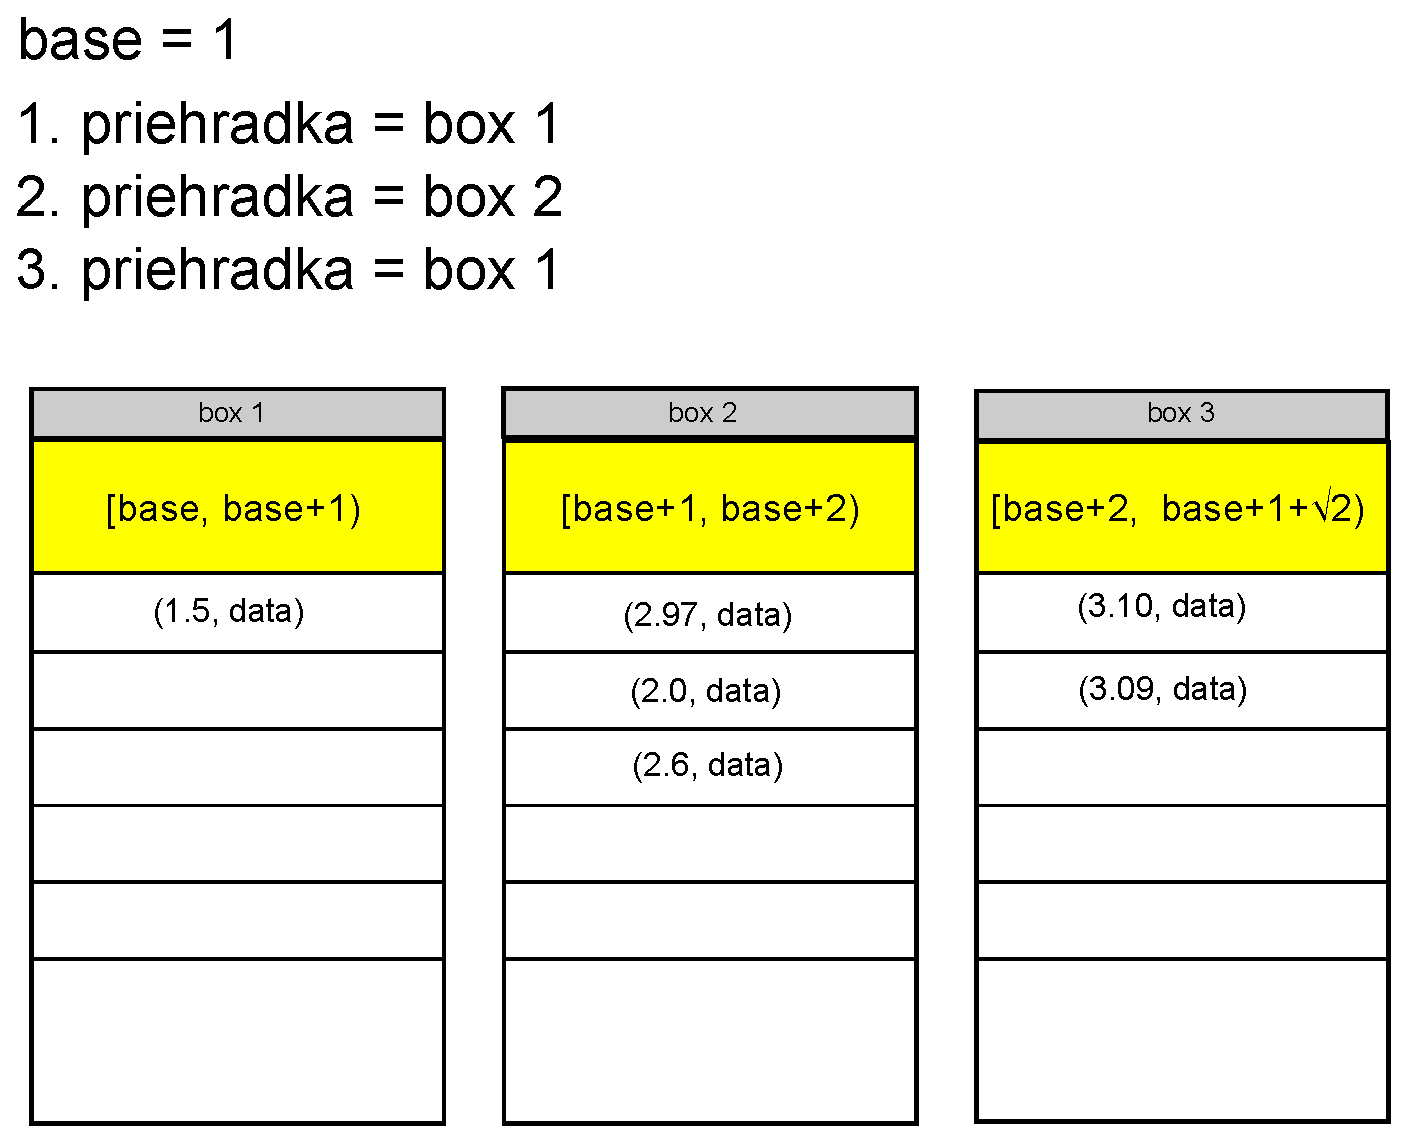
\includegraphics[width=\textwidth]{./img/priehradky_naplnene_default_i.eps}
\caption{Insert}
\label{fig:priehradky_i}
\end{figure}


Zmazanie prvku vidíme na obrázku \ref{fig:priehradky_i_d1}.
Celé zmazanie spočíva v inkrementácii ukazovateľa na vrch priehradky.

\begin{figure}[h]
\centering
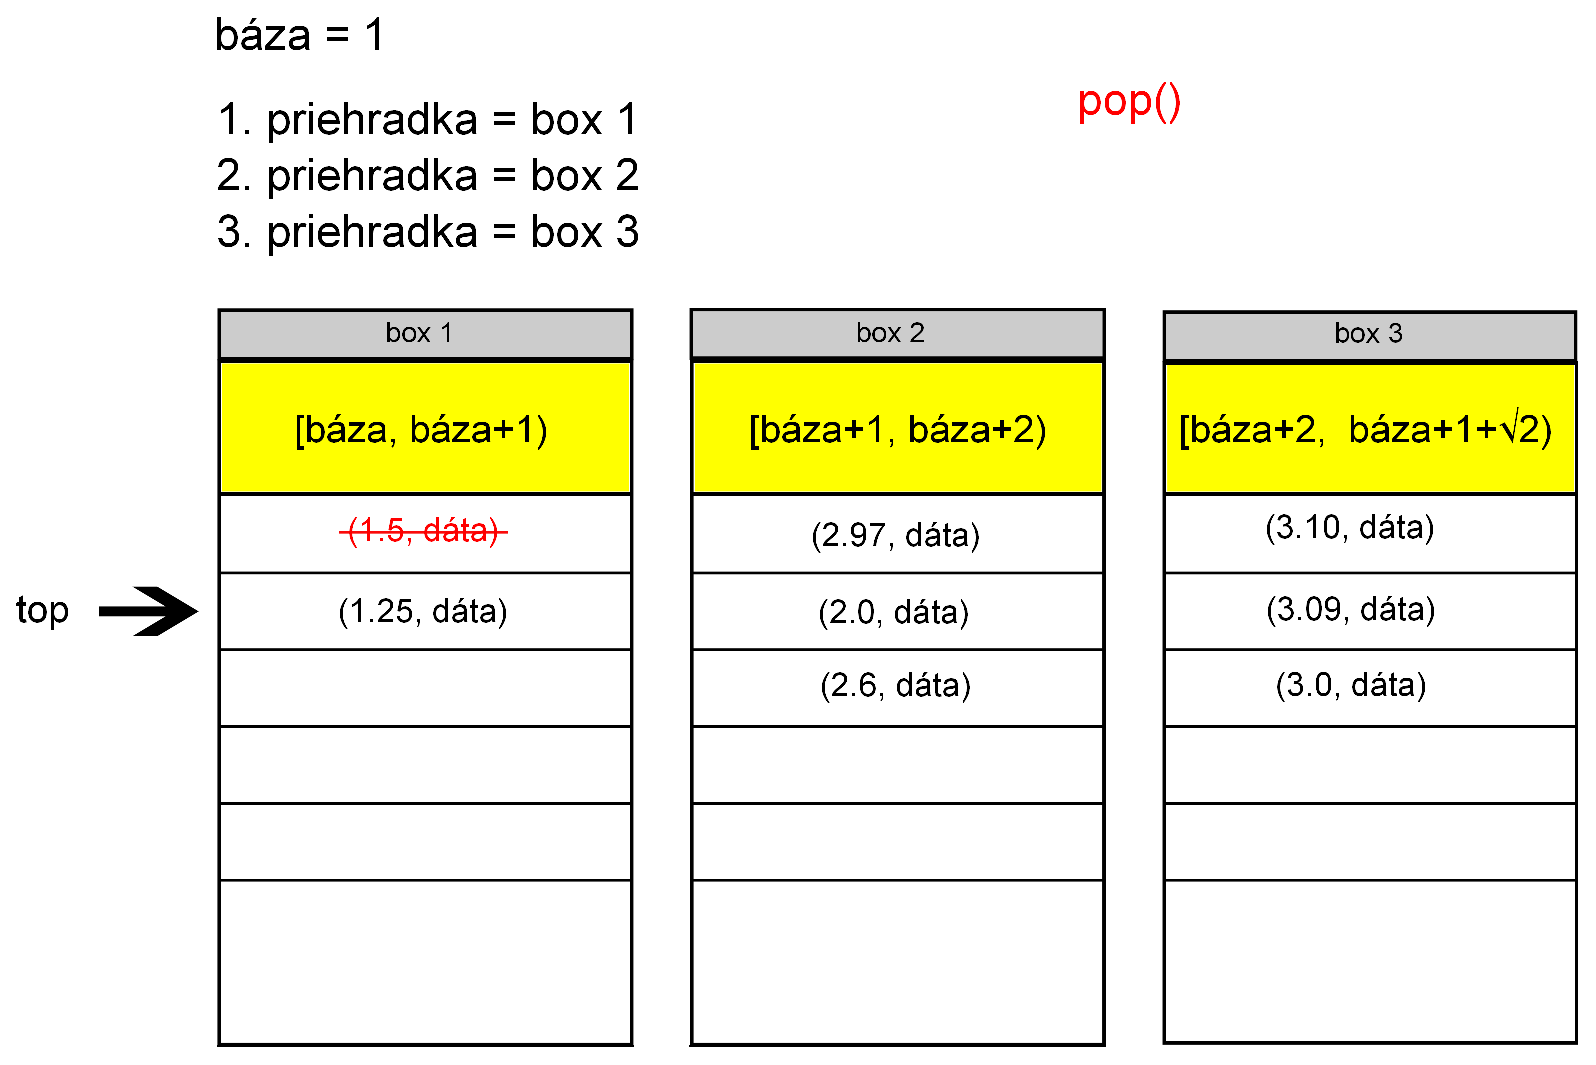
\includegraphics[width=\textwidth]{./img/priehradky_naplnene_default_i_d1.eps}
\caption{Pop (1)}
\label{fig:priehradky_i_d1}
\end{figure}


Pokiaľ sa v priehradke nachádza jediný prvok a ten chceme vybrať, tak nám inkrementácia premennej $ top $ v priehradke 
nepostačí. Musíme prehodiť priehradky. Druhú priehradku presunúť
na miesto prvej, tretiu na miesto druhej a prvú umiestniť nakoniec. Viď obrázok \ref{fig:priehradky_i_d2}. Nakoniec musíme zvýšit bázickú vzdialenosť. Zmena poradia týchto priehradok sa samozrejme uskutočňuje cez prehodenie smerníkov.
Keďže máme konštatný počet priehradok, tak aj táto operácia
trvá konštantný čas.

\begin{figure}[h]
\centering
\includegraphics[width=\textwidth]{./img/priehradky_naplnene_default_i_d2.eps}
\caption{Pop (2)}
\label{fig:priehradky_i_d2}
\end{figure}


\begin{theorem}[korektnosť priehradkovej štruktúry]
Dijkstrov algoritmu používajúci haldu $BucketHeap$ vráti korektné najkratšie vzdialenosti do vrcholov grafu.
\end{theorem}
\begin{proof}
Rozsah každej priehradky je ostro menší, ako 1. To znamená, že podľa príkladu \ref{ex:range} operácia $pop()$ vracia prvky v poradí, ktoré
nepokazí chod algoritmu. 

Treba ešte dokázať, že tri priehradky postačujú. To je zrejmé,
pretože keď vyberieme vrchol z prvej priehradky, tak jeho vzdialenosť je v rozsahu $[b, b+1)$. Keď prechádzame jeho susedné vrcholy, tak najdlhšia hrana je $ \sqrt{2} $ a teda vzdialenosť k najvzdialenejšiemu susednému vrcholu je ostro menšia, ako $b+1+\sqrt{2}$.
\end{proof}


\section{A*}
Ďalší algoritmus, ktorým sa budeme zaoberať je algoritmus
A* \cite{astar72} prvykrát popísaný v roku 1968.

Tento algoritmus vychádza z Dijkstrovho algoritmu a je mu veľmi podobný. Hlavný rozdiel medzi týmito algoritmami je, že
kým Dijkstrov algoritmus vyberá z haldy vrcholy s neklesajúcou vzdialenosťou $ d(v) $ od počiatku, tak algoritmus A* vyberá prvky s neklesajúcou vzdialenosťou $ f(v) := d(s,v) + h(v,t) $, kde $ h(v, t) $ značí heuristickú funkciu, ktorá je dolným odhadom vzdialenosti od vrcholu $ v $ do cieľa $ t $. Obrátene, Dijkstrov algoritmus si vieme predstaviť ako algoritmus A*, kde $ \forall v \in G: h(v, t) = 0 $.

Použitá heuristická funkcia má dopad na počet prehľadaných vrcholov a teda do zásadnej miery ovplyvňuje výkon algoritmu.

\subsection{Heuristická funkcia}
 Heuristická funkcia nemôže byť ľubovoľná. Funkcia musí predstavovať tzv. {\sl prípustný potenciál}. Podrobnejší popis sa nachádza napr. na \cite{mares07} \cite{golberg01} \cite{goldbergharrelson05}. Ďalej sa budeme venovať len funkciám, ktoré túto podmienku splňujú.


Najčastejšie heuristické funkcie sú tieto:

\begin{itemize}
\item Euklidovská vzdialenosť.
\item Trojuholníková nerovnosť, tzv. $ landmarks $.
\end{itemize}


\paragraph{Euklidovská vzdialenosť}

Euklidovská vzdialenosť je najjednoduchšie implementovateľná heuristická funkcia. Na väčšine jednoduchých grafov s malým počtom prekážok vracia dobré výsledky. Problém nastáva na grafoch, kde začiatok a koniec cesty sú geometricky blízko seba, hoci ich skutočná vzdialenosť je veľká.
Príklad vidíme na obrázku \ref{fig:antieuclid}.
TODO?? pozor na blbe rozdelenie obdlznikov - ja to ratam 
aj cez sikme hrany atd atd


\begin{figure}[h]
\centering
\includegraphics[width=0.5\textwidth]{./img/antieuclid505d.jpg}
\caption{Mapa, na ktorej euklidovská heuristika zlyhá.}
\label{fig:antieuclid}
\end{figure}


\paragraph{Landmarks a trojuholníková nerovnosť}
Nevýhoda použitia euklidovskej heuristickej funkcie je na obecných mapách zjavná. To motivovalo vymyslieť heuristiku, ktorá lepšie odráža vzdialenosti v grafe.

Jednou z týchto heuristík je počítanie dolného odhadu pomocou tzv. {\sl landmarks}. 

Landmarks sú vybrané vrcholy v grafe, z ktorých je následne prepočítaná najkratšia vzdialenosť do všetkych ostatných
vrcholov grafu. 



Kedže jeden prechod grafu vieme Dijkstrovým algoritmom s priehradkami vykonať za lineárny čas, predpočítanie $ k $ landmarkov trvá $ \BigO{kn} $, kde $n$ značí počet vrcholov grafu.


TODO?? ako to funguje...

\subparagraph{Možnosti voľby landmarkov}

Pri voľbe landmarkov sú dva faktory: počet a rozmiestnenie.

\begin{example}[na počte záleží]
Pokiaľ zvolíme málo landmarkov, tak dolný odhad nebude presný.
Pokiaľ ich zvolíme priveľa, tak prepočet vzdialenosti cez každý landmark pre každý vrchol zaberie veľa času.
\end{example}

\begin{example}[na rozmiestnení záleží]
Pokiaľ zvolíme všetky landmarky hneď pri sebe, tak heuristika
nám nebude vraciať dostatočne presné dolné odhady na vzdialenosť vrcholov, ktoré sú ďaleko od landmarkov.
\end{example}


TODO??potencialy euklid landmarks landmark selection priblem s priehradkami
\part{Implementácia}
\chapter{Nový algoritmus: NovellA*}

\section{Zlepšenie výkonu v niektorých prípadoch}
Nie všetky najkratšie cesty ale musia obchádzať veľa prekážok. 
V mnohých prípadoch nemusí medzi počiatočným a koncovým bodom ležať žiadna prekážka, a teda cesty sú veľmi priamočiare. To sa pokúsime využiť na~zlepšenie výkonu algoritmu.
 
Pre ľahšie vyjadrovanie si zaveďme definíciu {\sl mriežkového grafu bez prekážok}.

\begin{define}
{\sl Mriežkový graf je bez prekážok} 
pokiaľ medzi každými dvoma susednými vrcholmi existuje hrana.
\end{define}


Kvôli lepšej prehľadnosti budeme mriežkový graf bez prekážok nazývať aj {\sl obdĺžnik}.
Intuitívne, kvôli jeho vizuálnej interpretácii.

Majme mriežkový graf bez prekážok a hľadajme najkratšiu cestu medzi bodmi $s=(x_s,y_s), t=(x_t,y_t)$.
V tomto prípade vieme nájsť najkratšiu cestu veľmi jednoducho.

\begin{algorithm}
\caption{Nájdi najkratšiu cestu medzi dvoma bodmi {\sl s} a {\sl t} na mriežkovom grafe bez prekážok}
\label{alg1}
\begin{algorithmic}[1] % number one = line numbering is on
\REQUIRE $s=(x_s,y_s), t=(x_t,y_t)$
\ENSURE $path$


\STATE path.append($(x_s, y_s)$)
\COMMENT {pridám počiatok}

\WHILE {$x_s \neq x_t \vee y_s \neq y_t $}
	\IF {$x_s < x_t$}
		\STATE $x_s \leftarrow x_s + 1$
	\ELSIF {$x_s > x_t$}
		\STATE $x_s \leftarrow x_s - 1$
	\ENDIF

	\IF {$y_s < y_t$}
		\STATE $y_s \leftarrow y_s + 1$
	\ELSIF {$y_s>y_t$}
		\STATE $y_s \leftarrow y_s - 1$
	\ENDIF
	\STATE path.append($(x_s, y_s)$)
\ENDWHILE

\end{algorithmic}
\end{algorithm}



Teda, jednoducho povedané: keď sa počiatočný a koncový bod líšia v jednej súradnici, tak sa posúvame priamočiaro,
keď sa líšia v oboch, tak sa posúvame šikmo.


Pokiaľ si zadefinujeme 
$ dx := |x_t - x_s|$ 
a
$ dy :=|y_t - y_s| $
 , tak počet vrcholov,
ktorými cesta prechádza vieme zhora odhadnúť, ako $\max(dx, dy)$. Jej vzdialenosť vieme zistiť v čase  $\BigO{\max(dx, dy)}$
Na zistenie vzdialenosti v každom kroku nám stači konštantná pamäť.

TODO?? Poznamka, ze nepotrebujem na to obdlzniky, mozem robit aj komplikovanejsie utvary, ale by to sa blbo hladalo... ledaze...

Skúsme to teda nejak využiť. Pokiaľ vieme, že počiatočný aj koncový bod ležia v jednom obdĺžniku, tak máme problém vyriešený. 
Jediným problémom ostalo takéto obdĺžniky nájsť. 


\section{Hľadáme obdĺžniky}


\subsection{Proporcie obdĺžnikov}
Dôležitou otázkou je, na akých vlastnostiach obdĺžnikov záleží. Uvažujme nasledujúci motivačný príklad.
\begin{example}
Majme na mape nájdené dva obdĺžniky, ktorých celkový obsah je 10.
Predstavme si tieto dva prípady. V prvom prípade je obsah prvého 9 a druhého 1, v druhom prípade sú obsahy 6 a 4. 
Chceme maximalizovať pravdepodobnosť toho, aby pri voľbe dvoch náhodných bodov boli obe v rovnakom obdĺžniku.
\end{example}


Úlohu vieme zobecniť na klasickú pravdepodobnostno-optimalizačnú úlohu.

\begin{example}
Majme {\sl k} ekvivalenčných tried na množine s {\sl n} prvkami. Ako zvoliť ekvivalenčné triedy tak, 
aby pri voľbe dvoch náhodných prvkov bola pravdepodobnosť toho, 
že oba prvky budú v tej istej ekvivalenčnej triede čo najvyššia?
\end{example}

\begin{note}
Ekvivalenčnú triedu predstavuje obdĺžnik a množinu predstavuje množina vrcholov grafu.
Alternatívne sa môžeme na úlohu pozerať ako na problém farbenia guličiek čo najmenším počtom farieb.
\end{note}

Zapíšme túto úlohu formálne.


Majme $n$-prvkovú množinu $Prv = \{x_1,\ldots,x_n\}$, $k$-prvkovú množinu ekvivalenčných tried $Ek = \{ek_1,\ldots, ek_k\}$, veľkosť 
triedy $\|ek_i\|$ označme $k_i$ a zaveďme funkciu $f \colon Prv \to Ek$ ktorá roztriedi prvky do ekvivalenčných tried.

Označme výberový priestor $\Omega = \{(x_a, x_b) | x_a, x_b \in Prv, a \not= b \}$
Udalosťou $A_i$ nazveme jav, v~ktorom oba prvky patria do tej istej ekvivalenčnej triedy $ek_i$,
teda $A_i = \{(x_a, x_b) | x_a, x_b \in Prv, a \not= b, f(x_a) = f(x_b) = ek_i \}$
Jav $A = \bigcup_{i=1}^{k} A_i$ teda nastáva práve vtedy,
 keď oba vybrané prvky patria do rovnakej triedy.

Úlohou je teda navrhnúť funkciu $f$ tak, aby pravdepodobnosť $P[A]$ bola čo najvyššia. 
Keďže udalosti $A_i$ sú nezlučiteľné, môžme písať 
$P[A] = P[\bigcup_{i \in Ek} A_i] = \sum_{i \in Ek}P[A_i]$.

Ak si pravdepodobnosť každého javu rozpíšeme, dostaneme 
$\sum_{i \in Ek}P[A_i] = \sum_{i = 1}^{k} \frac{{{k_i} \choose {2}}}{{{|Prv|} \choose {2}}}$.


nakoľko chceme nejak rozvrhnúť prvky v triedach $ek_i$, a menovateľ je len
konštanta, môžme ho vynechať.

Maximalizujeme teda hodnotu výrazu 
$\sum_{i = 1}^{k} {{k_i} \choose {2}} = \sum_{i = 1}^{k} {\frac{k_i!}{(k_i -2 )!2!}} = \sum_{i = 1}^{k}{\frac{k_i (k_i-1)}{2}}$.
Po vyškrtnutí konštanty a roznásobení sme dostali nasledujúcu optimalizačnú úlohu:
maximalizovať $\sum_{i = 1}^{k} {k_i^2 - k_i}$ za podmienok $\sum_{k=1}^{k}k_i = n$,
kde $k_i \in \N_0$.

Sumu si vieme rozpísať ako 
$\sum_{i = 1}^{k} {k_i^2 - k_i} = \sum_{i = 1}^{k} {k_i^2} + \sum_{i = 1}^{k}{-k_i}$
druhá suma sa nasčíta $-n$, čo je konštanta, takže nám stačí maximalizovať 
$\sum_{i = 1}^{k} {k_i^2}$.

Teraz nám už len zostáva použiť nerovnosť
$(a+b)^2 \geq a^2 + b^2$ ktorá platí pre $a,b \geq 0$, z ktorej jasne vyplýva, že potrebujeme spraviť ľubovoľné $k_i$ čo najväčšie.
Ekvivalenčné triedy musia teda byť čo najväčšie a problém sa transformuje na problém hľadania
obdĺžnikov s najväčším možným obsahom.
V programe tento problém rieši trieda Colorizator.


\subsection{Nájdenie najväčšej jednotkovej podmatice}
Ako sme si v úvode povedali, mriežkovú mapu vieme reprezentovať ako maticu a teda
problém môžeme ekvivalentne zapísať ako problém hľadania najväčšej jednotkovej podmatice.
Tento problém má riešenie v čase lineárnom od počtu vrcholov a teda nájdenie $k$ najväčších
jednotkových matíc trvá $\BigO{k*n}$, kde n je počet vrcholov matice.

Slovný popis algoritmu \ref{alg:largest_submatrix}: 
V prvom prechode maticou si u každého vrcholu zapamätáme počet jedničiek naľavo od neho, vratane daneho vrcholu. 
Tento prechod trvá lineárny čas.

V druhom prechode treba prejsť zaradom všetky stĺpce zľava doprava



\begin{algorithm}
\caption{Nájdenie najväčšej jednotkovej podmatice v matici  $m$x$n$}
\label{alg:largest_submatrix}
\begin{algorithmic}[1] % number one = line numbering is on
\REQUIRE matica $M$ rozmerov $m x n$ nad telesom $\Z_2$
\ENSURE pravý dolný roh podmatice aj s jej rozmermi


\FORALL {prvok $p$, $p \in M$}
	\IF {$p = 0$}
		\STATE nalavoOdPrvku(p) $\leftarrow$ 0
	\ELSE
		\STATE nalavoOdPrvku(p) $\leftarrow$ najdlhšia súvislá postupnosť jednotiek končiaca prvkom $p$
	\ENDIF	
\ENDFOR

\FOR {stĺpec $s$, $s \in M$ }
	\STATE Vytvor nový zásobník dvojíc (riadok, nalavoOdPrvku)
	\FOR {riadok $r$, $r \in M$ }
		\STATE $p \leftarrow (s, r)$
		
		\WHILE {Zásobník je neprázdny}
			\STATE vyberiem prvok $top$ z vrcholu zásobníka
			\IF {$top$ . nalavoOdPrvku $>$ nalavoOdPrvku(p)}
						
				\STATE prvokZoZasobnika $\leftarrow$ ($top$.r, s)
				\STATE DlzkaSekvencie(prvokZoZasobnika) = r - prvokZoZasobnika.r
			
			\ELSE
				\STATE Vložím prvok $prvokZoZasobnika$ do zásobníka
				\STATE break
			\ENDIF
		\ENDWHILE
		
		\STATE Do zásobníka vložím dvojicu (r, nalavoOdPrvku(p))
	\ENDFOR
	
	\WHILE {Zásobník je neprázdny}
		\STATE vyberiem prvok $top$ z vrcholu zásobníka
		\STATE prvokZoZasobnika $\leftarrow$ ($top$.r, s)
		\STATE DlzkaSekvencie(prvokZoZasobnika) = m - prvokZoZasobnika.r
		
	\ENDWHILE
\ENDFOR




\end{algorithmic}
\end{algorithm}

\chapter{Testovanie a výsledky}

\section{Kritériá a popis testovania}
\subsection{Vstupné dáta}
Častým problémom pri vzájomnom porovnávaní algoritmov je
nájsť testovaciu vzorku, ktorá mi otestovala beh algoritmu na širokej škále grafov.
Ako bolo v úvode spomenuté, súťaž {\sl Grid-Based Path Planning Competition} poskytuje množstvo máp rôznych typov a rozmerov,
na ktorých sa algoritmy dajú testovať. Konkrétny popis typov máp sa nachádza v \cite{sturtevant2012benchmarks}.

\subsection{Testovacie kritériá}
Testovacie kritéria budú podobné ako testovacie kritériá v súťaži. Budú sa však mierne líšiť, pretože algoritmus nebol 
naplánovaný tak, aby .... TODO?? (prvych 20 kroko a nezaujima, na druhu stranu ma zaujima pocet prehladanych vrcholov...)

\begin{itemize}
\item Počet prehľadaných vrcholov.
\item Rýchlosť nájdenia cesty.
\end{itemize}


\subsection{Testované algoritmy}
Testovať budeme nasledujúce algoritmy:
\begin{itemize}
\item Dijkstrov algoritmus nad binárnou haldou.
\item Dijkstrov algoritmus nad priehradkovou haldou.
\item A* používajúc rôzny počet landmarkov.
\item A* používajú optimálny počet landmarkov a obdĺžnikovú dekompozíciu.
\item TODO?? nieco dalsie blablabla - cudzie algoritmy.
\end{itemize}


\subsection{Kompilácia}
Kód bude kompilovaný kompilátorom g++. Bude porovnaná
rýchlosť behu programu pri kompilácii s týmito direktívami.
\begin{itemize}
\item -O1
\item -O2
\item -O3
\item -O3 -march=native
\end{itemize}
ASK?? toto bude len pri jednom algoritme pri jednom grafe, nie? neni to zbytocne???

\subsection{Typy map a ciest}
TODO?? - kratke dlhe, klukate a rovne obrazok asopn 3 map





(ASK?? poet prehladanych vrcholov nie je kriterium, ktore dokazem testovat na cudzich algoritmoch - musel by smo do nich zahat a pridavat tam funkciu, ktora to pocita - co mam robit? mam pocet vrcholov testovat len na mojich algoritmoch?)




Na porovnávanie využijeme benchmark

TODO?? bibliografia styl - priezvisko,meno - alebo naopak???
\chapter{T-maps - Vizuálna predstava}

Pre názornejšiu predstavu behu algoritmu sme navrhli softvér \textbf{T-maps}, ktorý beh algoritmov ilustruje graficky.

\section{Použitie}

Program T-maps má funčnosť veľmi podobnú programu Goole Maps. Na začiatku do neho nahrajeme mapu, nad ktorou algoritmus beží a taktiež dáta
tohto algoritmu (prehľadané vrcholy a najkratšiu cestu) a program tieto hodnoty graficky znázorní.
Medzi možnosti programu patrí export mapy a viditeľného poľa do súboru.
 TODO??  uzivatelska dokumentacia
Mozno popis zaujimavej casti  


% Ukázka použití některých konstrukcí LateXu (odkomentujte, chcete-li)
%%%% Ukázka použití některých konstrukcí LaTeXu

\subsection{Ukázka \LaTeX{}u}
\label{ssec:ukazka}

V~této krátké části ukážeme použití několika základních konstrukcí \LaTeX{}u,
které by se vám mohly při psaní práce hodit.

Třeba odrážky:

\begin{itemize}
\item Logo Matfyzu vidíme na obrázku.~\ref{fig:mff}
\item Tato subsekce má číslo~\ref{ssec:ukazka}.
\item Odkaz na literaturu~\cite{lamport94}.
\end{itemize}

Druhy pomlček:
červeno-černý (krátká),
strana 16--22 (střední),
$45-44$ (minus),
a~toto je --- jak se asi dalo čekat --- vložená věta ohraničená dlouhými pomlčkami.
(Všimněte si, že jsme za \verb|a| napsali vlnovku místo mezery: to aby se
tam nemohl rozdělit řádek.)

% Makro na české uvozovky (novější verze LaTeXu ho už mají zabudované)
%\newcommand{\uv}[1]{\quotedblbase #1\textquotedblleft}
\uv{České uvozovky.}

%\newtheorem{theorem}{Věta}
%\newtheorem*{define}{Definice}	% Definice nečíslujeme, proto "*"

\begin{define}
{\sl Strom} je souvislý graf bez kružnic.
\end{define}


\begin{theorem}
Tato věta neplatí.
\end{theorem}


\begin{proof}
Neplatné věty nemají důkaz.
\end{proof}

\cite{cfsimpl}


\begin{figure}
	\centering
	\includegraphics[width=30mm]{./img/logo.eps}
	\caption{Logo MFF UK}
	\label{fig:mff}
\end{figure}

\begin{algorithm}
\DontPrintSemicolon % Some LaTeX compilers require you to use \dontprintsemicolon instead 
\KwIn{A set $C = \{c_1, c_2, \ldots, c_r\}$ of denominations of coins, where $c_i > c_2 > \ldots > c_r$ and a positive number $n$}
\KwOut{A list of coins $d_1,d_2,\ldots,d_k$, such that $\sum_{i=1}^k d_i = n$ and $k$ is minimized}
$C \gets \emptyset$\;
\For{$i \gets 1$ \textbf{to} $r$}{
  \While{$n \geq c_i$} {
    $C \gets C \cup \{c_i\}$\;
    $n \gets n - c_i$\;
  }
}
\Return{$C$}\;
\caption{{\sc Change} Makes change using the smallest number of coins}
\label{algo:change}
\end{algorithm}

Algorithm~\ref{algo:duplicate} and Algorithm~\ref{algo:duplicate2} will
find the first duplicate element in a sequence of integers.

\begin{algorithm}
\DontPrintSemicolon % Some LaTeX compilers require you to use \dontprintsemicolon instead
\KwIn{A sequence of integers $\langle a_1, a_2, \ldots, a_n \rangle$}
\KwOut{The index of first location witht he same value as in a previous location in the sequence}
$location \gets 0$\;
$i \gets 2$\;
\While{$i \leq n$ \textbf{and} $location = 0$}{
  $j \gets 1$\;
  \While{$j < i$ \textbf{and} $location = 0$}{
    % The "u" before the "If" makes it so there is no "end" after the statement, so the else will then follow
    \uIf{$a_i = a_j$}{
      $location \gets i$\;
    }
    \Else{
      $j \gets j + 1$\;
    }
  }
  $i \gets i + 1$\;
}
\Return{location}\;
\caption{{\sc FindDuplicate}}
\label{algo:duplicate}
\end{algorithm}

\begin{algorithm}
\DontPrintSemicolon
\KwIn{A sequence of integers $\langle a_1, a_2, \ldots, a_n \rangle$}
\KwOut{The index of first location witht he same value as in a previous location in the sequence}
$location \gets 0$\;
$i \gets 2$\;
\While{$i \leq n \land location = 0$}{
  $j \gets 1$\;
  \While{$j < i \land location = 0$}{
    % The "l" before the If makes it so it does not expand to a second line
    \lIf{$a_i = a_j$}{
      $location \gets i$\;
    }
    \lElse{
      $j \gets j + 1$\;
    }
  }
  $i \gets i + 1$\;
}
\Return{location}\;
\caption{{\sc FindDuplicate2}}
\label{algo:duplicate2}
\end{algorithm}

\chapter*{Záver}
\addcontentsline{toc}{chapter}{Záver}

Práca sa zaoberala hľadaním ciest na mriežkových grafoch s dôrazom na rýchlosť nájdenia cesty a~dĺžku nájdenej cesty. 

V prvej časti práca podala prehľad najdôležitejších algoritmov používaných pri hľadaní ciest. Kľúčovým algoritmom je Dijkstrov algoritmus. Postupnými vylepšeniami a~optimalizáciami na mriežkové grafy bol následne skonštruovaný vylepšený Dijkstrov algoritmus bežiaci v lineárnom čase. 
Ďalším dôležitých algoritmom je algoritmus A*. V práci bol popísaný a naprogramovaný s rôznymi heuristikami.

V druhej časti bol zavedený nový pohľad na analýzu mriežkového grafu --- jeho dekompozícia na obdĺžniky. 
Pomocou nej bolo možné na grafoch s veľkým počtom hrán vyhľadávať cestu efektívnejšie, ako doterajšími spôsobmi.
Algoritmus navrhnutý v tejto časti vychádza z Algoritmu A*, používa landmarky a taktiež túto dekompozíciu na obdĺžniky.

Vo štvrtej kapitole sme spravili porovnanie doterajších algoritmov s týmto novým algoritmom. Vo výsledkoch sme zistili, 
že tento algoritmus poskytuje viditeľné zrýchlenie, pri vyhľadávaní cesty medzi vrcholmi, ktorých vzdialenosť je malá. Z tohto dôvodu navrhujeme začleniť túto metódu do ostatných vyhľadávacích algoritmov, ktoré často hľadajú cestu medzi blízkymi bodmi v mriežkových grafoch s veľkým množstvom hrán.

Práca taktiež ukázala, že nižšia asymptotická zložitosť neznamená vyššiu reálnu rýchlost behu. Taktiež poukázala na to, že hoci algoritmus A* vie orezať počet prehľadaných vrcholov až na tretinu, neznamená to ešte aj vyššiu celkovú rýchlosť behu.


%%% Seznam použité literatury
%%% Seznam použité literatury je zpracován podle platných standardů. Povinnou citační
%%% normou pro bakalářskou práci je ISO 690. Jména časopisů lze uvádět zkráceně, ale jen
%%% v kodifikované podobě. Všechny použité zdroje a prameny musí být řádně citovány.

\def\bibname{Zoznam použitej literatúry}
\begin{thebibliography}{99}
\addcontentsline{toc}{chapter}{\bibname}
%%%%

\bibitem{euler41}
	L. Euler. 
	\emph{Solutio problematis ad geometriam situs pertinentis}.
    Commentarii academiae scientiarum Petropolitanae, 8:128–140, 1741.

\bibitem{dijkstra59}
  E. W. Dijkstra.
  \emph{A note on two problems in connexion with graphs}.
  Numerische Mathematik, 1(1):269--271, 1959.

\bibitem{floyd62}
R.~W. Floyd.
\newblock Algorithm 97: Shortest path.
\newblock {\em Commun. ACM}, 5(6):345--, June 1962.



\bibitem{mares07}
  M. Mareš.
  \emph{Krajinou grafových algoritmů}.
  ITI Series, Prague 2007 [ONLINE]. [CIT. 2013-7-21]. Dostupné z \url{http:
  //mj.ucw.cz/vyuka/ga/}.
  
\bibitem{astar72}
P.~E. Hart, N.~J. Nilsson, B. Raphael.
\newblock Correction to a formal basis for the heuristic determination of minimum cost paths.
\newblock {\em SIGART Bull.}, (37):28--29, December 1972.

\bibitem{golberg01}
A. V. Goldberg. 
\emph{Shortest Path Algorithms: Engineering Aspects}. 
In Proc. ESAAC '01, Lecture Notes in
Computer Science. Springer-Verlag, 2001.


\bibitem{goldbergharrelson05}
A. V. Goldberg, C. Harrelson. 
\emph{Computing the Shortest Path: A* Search Meets Graph Theory}.
In Proc. 16th ACM-SIAM Symposium on Discrete Algorithms, pages 156--165, 2005.

\bibitem{asymptotic65}
 J. Hartmanis, R. Stearns. 
 \emph{On the computational complexity of algorithms}. 
 Transactions of the American Mathematical Society, vol. 117, 285--306, 1965.

\bibitem{sturtevantgppc}
  N.~Sturtevant.
  \emph{GPPC: Grid-Based Path Planning Competition} [ONLINE] 2013. [CIT. 2013-7-21].
  Dostupné z: \url{http://movingai.com/GPPC/}. 
   
\bibitem{sturtevant2012benchmarks}
N.~Sturtevant.
\newblock Benchmarks for grid-based pathfinding.
\newblock {\em Transactions on Computational Intelligence and AI in Games},
  4(2):144 -- 148, 2012.
   
\bibitem{gs97}
A.~Goldberg, C. Silverstein.
\emph{Implementations of Dijkstra’s Algorithm Based on Multi-Level Buckets}.
Springer Berlin Heidelberg,
1997.

\bibitem{krasner_mvc_1988}
G.~Krasner, S.~Pope.
\newblock A description of the {Model-View-Controller} user interface paradigm
  in the smalltalk-80 system.
\newblock {\em Journal of Object Oriented Programming}, 1(3):26--49, 1988.

\bibitem{agrawal_largest_submatrix}
A. Agrawal.
\emph{Find largest sub-matrix with all 1s (not necessarily square)} [ONLINE] 2011. [CIT. 2013-7-21]. Dostupné z
\url{http://tech-queries.blogspot.cz/2011/09/find-largest-sub-matrix-with-all-1s-not.html}





\end{thebibliography}


%%% Tabulky v bakalářské práci, existují-li.
\chapwithtoc{Zoznam tabuliek}

%%% Použité zkratky v bakalářské práci, existují-li, včetně jejich vysvětlení.
\chapwithtoc{Zoznam použitých skratiek}

%%% Přílohy k bakalářské práci, existují-li (různé dodatky jako výpisy programů,
%%% diagramy apod.). Každá příloha musí být alespoň jednou odkazována z vlastního
%%% textu práce. Přílohy se číslují.
\chapwithtoc{Prílohy}

\openright
\end{document}
